\chapter{Konzeption}
\label{chap:konzeption}

Zur Erstellung des Konzepts gilt es mehrere Aspekte im Voraus genauer zu betrachten.
Dabei wird als erstes in \Cref{sec:weristmeinezielgruppe} die Zielgruppe der Softwarelösung analysiert. Daraufhin
wird in \Cref{sec:anforderungsanalyse} die Anforderungsanalyse der vier Aspekte; Gestaltung, Funktionalität,
Flexibilität und Codebasis behandelt. Nach der Anforderungsanalyse gilt es
in \Cref{sec:auswertungvorhandenersoftwareloesungen} die aktuelle Lage
des Marktes zu analysieren. Tools im Bereich der Geschäftsanalytik gibt es viele. \cite{WikiBISoftware}
Was zeichnet diese Softwarelösungen aus? Mit welchen Merkmalen kann man sich von vorhandenen Lösungen
bewusst unterscheiden? In \Cref{sec:progressivewebapp} und \ref{sec:microservices} beschäftigt
sich die Arbeit mit der Analyse zweier für die Softwarelösung relevanter Technologien.
Bei der ersten Technologie handelt es sich um eine Progressive Web App. Hier gilt es folgende
Fragen zu beantworten: Was ist eine Progressive Web App und macht diese 
im Kontext der Benutzeranforderungen Sinn? Was sind Vor- und Nachteile gegenüber nativer Apps?
Wie sieht es mit der Unterstützung der Plattformen aus? Als zweites wird ein für die
Serverinfrastruktur relevantes Architekturmuster als Lösungsansatz diskutiert. Hierbei
stellen sich folgende Leitfragen: Was versteht man unter Microservices? Macht eine
Microservice-Infrastruktur in Bezug auf die davor behandelten Anforderungen an die
Softwarelösung Sinn?

Sind all diese Fragen beantwortet, kann ein Grundkonzept der Gesamtanwendung entwickelt werden.
Hierbei werden in \Cref{sec:zielsetzung} die Ziele für die Softwarelösung gesetzt. In \Cref{sec:entwurf}
werden daraufhin Entwürfe sowohl von der Benutzeroberfläche als auch von der Infrastruktur vorgestellt.
Weitere Designentscheidungen werden in den folgenden Kapiteln debattiert.

\section{Wer ist die Zielgruppe?}
\label{sec:weristmeinezielgruppe}
Die in der Masterarbeit zu entwickelnde Softwarelösungen
soll den Bestandkunden von GBO Datacomp eine moderne Alternative geben, Daten 
auf mobilen Endgeräten wie Tablets, Smartphones aber auch Desktop PCs auswerten zu können.
Desweiteren muss die Software Neukunden ansprechen und zum Kauf überzeugen. GBO Datacomp
hat Kunden in vielen verschiedenen Branchen. So hat das Unternehmen Kunden in der
Automobilindustrie, in der Metall- und Gussindustrie, in der Lebensmittelindustrie,
in der Steinverarbeitung, in der Verpackungsindustrie, in dem Druckgewerbe, in der
Zahntechnik, der Kundstoffverarbeitung, Holzindustrie, Möbelindustrie, Metall- und Gussindustrie sowie
der Steinverarbeitung.\cite{GBODatacompBranchenloesungen}

Eines der wichtigsten Produkte von GBO Datacomp ist BisoftMES, eine Software zur Erfassung von
Maschinen- und Betriebsdaten. Diese Daten können Auftragsdaten, Schichtdaten und Maschinendaten sein.
So können die Benutzer der Software Trendanalysen durchführen, Schicht- und Maschinendaten vergleichen und
Leistungskennzahlen auswerten, um so möglichen Störungen und Ausfällen im Betrieb vorzubeugen.

Wer genau wird das agile Dashboard zur Betriebs- und Maschinendatenauswertung
benutzen? Dies kann sich je nach Betrieb unterscheiden. So interagieren von der
Managementebene aus über den Produktionsleiter bis hin zum Schichtarbeiter Benutzer mit dem
Dashboard. Eines der Dashboards könnte an einem speziell für die Softwarelösung
installierten Bildschirm in einer Produktionshalle angezeigt werden. Anderenfalls könnte aber
auch der Produktionsleiter in der Mittagspause mit seinem Handy die aktuellen Leistungskennzahlen 
(KPIs) abrufen. Viele Produktionshallen besitzen alte Windows-Rechner, die nicht
mit den neusten Browsern ausgestattet sind. Andere Betriebe besitzen Endgeräte mit Touchscreens.
Fassen wir all diese möglichen Szenarien zusammen, wird uns eines sehr deutlich. Von der
Softwarelösung wird eine gewisse Flexibilität abverlangt, die nicht zu unterschätzen ist.

\section{Anforderungsanalyse}
\label{sec:anforderungsanalyse}

In der Anforderungsanalyse soll es darum gehen, Anforderungen an die Software zu erkennen
und diese zu erörtern. Dabei werden die Anforderungen in vier Rubriken unterteilt. Als erstes werden 
in \Cref{subsec:gestaltung} die Anforderungen an die Gestaltung der Anwendung
gestellt. Hier geht es um das Aussehen sowie die Benutzerfreundlichkeit der Frontendanwendung.
Als zweites werden in \Cref{subsec:funktionalitaet} die Anforderungen an die Funktionalität der
Software analysiert. Was sind typische Benutzerhandlungen, die die Software ermöglichen
muss? Als drittes werden in \Cref{subsec:flexibilitaet} die Anforderungen zur Flexibilität
der Software erörtert. Im Unterschied zu den Anforderungen an die Funktionalität liegt hier
ein besonderer Fokus auf der Vielfalt bestimmter Funktionalitäten. Dabei stellt sich die Frage,
wie flexibel die Software in Bezug auf die zu analysierenden Daten und derer Visualisierung sein muss.
Als viertes werden in \Cref{subsec:codebasis} die Anforderungen an die Codebasis gestellt.
Hier geht es um die Qualitäten der Software. Es stellt sich die Frage, wie es mit den
Anforderungen an die Weiterverwendbarkeit sowie die Veränderbarkeit der Software aussieht.

GBO Datacomp hat seinerseits Anforderungen an die Software in Form eines Informationsblattes
bereitgestellt. Diese Anforderungen werden in den Folgeabschnitten miteinbezogen.

\subsection{Gestaltung}
\label{subsec:gestaltung}
Welche Anforderungen gibt es bei der Gestaltung der Anwendung oder noch spezieller 
der grafischen Oberfläche zu beachten? Wie bereits in der Zielgruppenanalyse
angemerkt, werden die verschiedensten Endgeräte auf die Software zugreifen.
GBO Datacomp erwähnt in ihrem Informationsblatt die Fokussierung auf folgende
drei Gerätetypen: Desktop-PCs, Tablets und Smartphones. Man kann davon ausgehen, dass die
Softwarelösung als Eingabeschnittstelle neben der Maus und der Tastatur auch mit einem Touchscreen
gesteuert werden kann. GBO Datacomp weißt speziell auf die unterschiedlichen Bildschirmgrößen
hin. So soll die Anwendung auf verschiedene Bildschirmgrößen reagieren und den Inhalt je nach
Größe zugänglich bereitstellen. Geräte des gleichen Typs weisen keine signifikanten Unterschiede
in der Darstellung auf. Um diese Anforderung umzusetzen, benötigt es neben der Erkennung
der Bildschirmgröße auch noch eine Erkennung des Gerätetyps.

Man kann davon ausgehen, dass neben den unterschiedlichen Gerätetypen auch unterschiedliche
Betriebssysteme verwendet werden. Laut StatCounter verteilt sich der weltweite Marktanteil
an Betriebssystemen laut einer Analyse vom Dezember 2019 wie folgt auf. Android führt mit
40,47\%, gefolgt von Windows mit 34,2\%, iOS mit 14,92\% und macOS mit 7,24\%. Linux mit 0,83\% und weitere
Betriebssysteme mit 1,24\% bilden hierbei eine Minderheit.\cite{StatCounterOSMarketShare} Betrachtet man den
Nutzungsanteil der Browser im Oktober 2019 weltweit, führt Chrome mit 64,92\%, gefolgt von Safari mit 15,97\%,
Firefox mit 4,33\%, Samsung Internet mit 3,29\%, der primär im asiatischen Bereich genutzte Browser UC
mit 2,94\%, Opera mit 2,34\%, Edge mit 2,05\%, Internet Explorer mit 1,98\%, Android mit 0,59\% und Sonstige mit 1,59\%.\cite{StatCounterBrowserMarketShare}
Diese Kennzahlen geben einen groben Überblick über die aktuelle Lage des Marktes. Der Markt wird klar von
Google und Microsoft Produkten dominiert. Allerdings variiert der Nutzungsanteil je nach Branche.
Um ein besseres Bild über die verwendeten Technologien möglicher Kunden zu erhalten,
lohnt es sich ein Blick auf die Produkte von GBO Datacomp selbst zu werfen.
BisoftMES, eines der zentralen Produkte von GBO Datacomp, "ist eine unter Microsoft.net
entwickelte Maschinen- und Betriebsdatenerfassungssoftware".\footnote{Aus dem BisoftMES Benutzerhandbuch\cite[S. 7]{BisoftMESHandbuch}}
Es liegt nahe, dass auch die Bestandskunden von GBO Datacomp Produkte aus der Microsoft
Produktpalette verwenden. Eine Unterstützung von Browsern wie Internet Explorer und Edge
wäre daher wünschenswert.

Die Anwendung sollte als Whitelabel Produkt eingesetzt werden können. Dies bedeutet soviel wie,
dass die GUI der Anwendung mit geringem Aufwand an das Erscheinungsbild eines Unternehmens angepasst
werden kann. Beispiele dafür gibt es in der Softwareindustrie häufig. So kann man bei
der Community Edition von Gitlab das Logo sowie das Farbschema der Anwendung in den Einstellungen
anpassen.\cite{GitlabDocs}

GBO Datacomp beschreibt in den Anforderungen des zu Beginn der Arbeit überreichten
Informationsblattes konkret, dass die Benutzbarkeit der Software ohne großen Schulungsaufwand möglich sein soll.
Dies steht im klaren Kontrast zu konkurrierenden Softwarelösungen im BI Sektor.
So bietet QlikTech, ein führendes Unternehmen im Bereich Business Intelligence,
weltweit Kurse für ihr Softwareprodukt Qlik Sense an. Die Kurse haben in der
Regel eine Zeitspanne zwischen drei bis fünf Tagen.\cite{QlikSenseTraining}
Dies ist auch verständlich angesichts der Tatsache, dass QlikTech in einigen
ihrer Produkte eine eigene SQL ähnliche Skriptsprache verwenden.\cite{QlikSenseScriptLanguage}
Um eine klare, selbsterklärende Gestaltung der Anwendung zu erlangen,
muss an der Komplexität der Funktionalität gespart werden. Des weiteren
gilt es darauf zu achten, dass eine klare Abstraktion der Funktionalitäten
gegeben ist. Um den Lernaufwand zu verringern, muss bekannte Technologien
der Erfindung neuer vorgezogen werden. Falls man jedoch beweisen kann,
dass die neu erfundene Technologie das im Fokus stehende Problem effizienter löst
sowie einfacher zu erlernen ist, spricht nichts dagegen, diese Technologie der bereits
etablierten Technologie vorzuziehen.

Fasst man die oben analysierten Anforderungen in Bezug auf die grafische Benutzeroberfläche
zusammen, kommt man auf folgendes: Die Benutzeroberfläche besitzt ein Responsive Design,
das sich auf die Gegebenheiten des jeweiligen Gerätes anpasst. Unterstützung
für die führenden Browser, Edge und Internet Explorer inbegriffen, ist gegeben.
Das Design ist mit wenig Aufwand an das Erscheinungsbild eines Unternehmens anpassbar.
Das GUI verfolgt eine klare, benutzerfreundliche Richtlinie.

\subsection{Funktionalität}
\label{subsec:funktionalitaet}
Die Analyse der Anforderungen an die Funktionalität der Software ist der
umfangreichste Teil der Anforderungsanalyse. Dabei gilt es folgende Frage zu beantworten:
Was sind die bedeutsamsten Anforderungen an die Funktionalität der Software?
Dazu muss man sich den Titel der Masterarbeit nochmal vor Augen führen.
Der Titel heißt: Agiles Dashboardingtool zur Datenvisualisierung
in einer Microservice-Infrastruktur. Die erste und bedeutsamste Funktionalität ist
die möglichst agile Erstellung eines Dashboards. Die Aufgabe des Dashboards ist es Daten
zu visualisieren. Um dies zu ermöglichen, benötigt das Dashboard Daten. Diese Daten
müssen aus einer Datenquelle geladen werden. GBO Datacomp stellt hierfür eine REST API
zur Verfügung. Für eine Datenquelle ist somit gesorgt. Um die Daten innerhalb der Anwendung
einem Dashboard zur Verfügung zu stellen, müssen die Daten zu einem passenden Format verarbeitet werden.
Zu guter Letzt muss noch definiert werden, welche Daten in welchem Dashboard verwendet
werden. Diese vier Funktionalitäten sind der Kern der Anwendung. In diesem Abschnitt
werden zuerst die Anforderungen der Kernfunktionalitäten genauer analysiert. Daraufhin werden die Anforderungen
für die Authentifizierung der Benutzer, die Rechteverwaltung, die Auswahl der Sprache,
die Navigation durch die Software, die Suche nach Ressourcen in der Anwendungen,
die Filterung der darzustellenden Daten im Dashboard sowie für die Möglichkeit,
die Anwendung auch offline zu verwenden, erörtert.

Was sind die Anforderungen für die Erstellung des agilen Dashboards? Wie bereits in dem
vorigen Abschnitt über die grafische Benutzeroberfläche debattiert, muss die Anwendung und
so auch die Erstellung des Dashboards selbsterklärend sein. Daraus resultiert, dass die Anwendung 
selbst die Justierung der einzelnen Komponenten des Dashboards übernimmt. Der
Benutzer kann in einem intuitiven Verfahren, einzelne Komponenten auswählen und diese
an bestimmte Positionen im Bildschirm ziehen. Desweiteren kann er die Komponenten
entfernen und ersetzen. Wirft man einen Blick auf andere BI Softwarelösungen,
stellt man fest, dass die Anzahl der Komponenten der Anwendung im Lauf der Zeit
stetig anwachsen kann. Somit ist die effiziente Auswahl, auch aus einer großen
Anzahl an Komponenten, pflicht.

Was sind die Anforderungen für das Laden der Daten in die Anwendung? Neben der Flexibilität,
die im darauffolgenden Abschnitt erörtert wird, muss das Laden von Daten schnell und zuverlässig
sein. Typische Vorgehensweisen der Anwender sind das Auswerten von Maschinendaten. Dabei kann es
sich um die Auslastung, Störfälle aber auch Ausfälle der Maschinen handeln. Es ist bedeutsam,
das der Anwender rechtzeitig von diesen Ereignissen informiert wird. Unsere
Aufmerksamkeit gilt also auch der zeitnahen Aktualisierung der Daten in den Dashboards. Nur
so kann sichergestellt werden, dass der Anwender auch zeitnah auf in den Daten erkenntliche
Ereignisse reagieren kann. In Anlehnung dieser Feststellung liegt es nahe, den Benutzer
über bestimmte Ereignisse per Benachrichtigung zu informieren. So kann man
eine Benachrichtigung auf das Smartphone des Benutzers schicken, sobald ein zuvor definierter
Schwellwert überschritten wird.

Welche Anforderungen sind für die Verarbeitung der Daten notwendig? Daten können Fehler oder Lücken
beinhalten. So kann in einer Spalte, die das ISO Datumsformat beinhalten, fälschlicherweise ein
ungültiger Wert vorkommen oder dieser komplett fehlen. Zugegebenermaßen reicht es für einen MVP, ein
minimal überlebensfähiges Produkt, aus, diese Unreinheiten so zu behandeln, dass die Anwendung
eine informationsreiche Fehlerwarnung an den Benutzer überliefert oder alternativ einen Standartwert
für fehlende Felder definiert.

Wie werden die Dashboards mit den nötigen Daten versorgt? Grundsätzlich ist klar davon auszugehen,
dass die Anwendung einen Zuweisungsmechanismus bereitstellt. Um von einer komplexeren, eingehenden
Datenstruktur zu einer für die Visualisierung geeigneten Datenstruktur zu kommen, müssen die gewollten
Daten ausgewählt und zugewiesen werden. Dem Benutzer selbst ist ein, ähnlich wie bei der Erstellung
des Dashboards, agiler Prozess zur Zuweisung der Daten ermöglicht. Ein Benutzer will auf einem
Dashboard unterschiedliche Quellen von Daten vergleichen. Somit muss die Möglichkeit bestehen,
unterschiedliche Zuweisungen für die Diagramme eines Dashboards zu tätigen.

Anschließend werden die Anforderungen für die Benutzerauthentifizierung und die Rechteverwaltung erörtert.
Sicherheit muss in jeder Anwendung, die mit Kundendaten interagiert, von großer Bedeutung sein.
Somit ist es naheliegend, dass für die heutigen IT-Sicherheitsstandards gesorgt wird. Progressive
Web Apps sind per Definition außerhalb der Entwicklung nur über HTTPS zu übertragen.\cite[S. 16]{KevinFrankPWAMasterarbeit}
OWASP (Open Web Application Security Project) veröffentlichte 2017 einen Bericht über die zehn
bedeutsamsten Sicherheitsrisiken von Webanwendungen. Darunter sind unter anderem die Einschleusung
von Quellcode durch mangelnde Maskierung, fehlerhafte Authentifizierungsverfahren, Preisgabe von sensiblen Daten,
XSS-Attacken und Fehlkonfigurationen von Sicherheitseinstellungen.\cite[S. 4]{OWASPTopTen}
Um die Kundendaten vor Angriffen zu schützen, liegt es nahe, dass diese Sicherheitsrisiken bei der
Entwicklung der Anwendung beachtet werden. Zum Funktionsumfang gehört dazu,
dass ein Benutzer ein Konto sicher anlegen, sich anmelden, abmelden und sein Konto auch wieder
löschen kann. Die Rechteverwaltung konzentriert sich laut GBO Datacomp vorerst auf die elementaren
Grundeigenschaften.

Da GBO Datacomp ihre Softwarelösungen auch an nicht deutschsprachige Kunden verkauft, ist es notwendig,
die Anwendung multilingual zu gestalten. Die Funktionalität, die Sprache der Anwendung zu verändern,
ist somit Teil der Anforderungen. Damit der Benutzer nicht bei jedem Besuch die Sprache neu einstellen
muss, gilt es die Spracheinstellungen im Browser zu persistieren. GBO Datacomp merkt hier an, dass diese
unabhängig von denen des Browsers gespeichert werden müssen.

Ein Benutzer will ohne großen Aufwand von einen Dashboard zu einem anderen gelangen. Er will kurz seine Profileinstellungen
einsehen, daraufhin an der Datenzuweisung arbeiten und dann die Dokumentation lesen.
Hierfür benötigt die Anwendung eine benutzerfreundliche Navigation. Ist die Anzahl der Ressourcen zu 
groß, muss die Anwendung einen automatischen Seitenumbruch einführen. Um die Suche nach speziellen
Ressourcen zu erleichtern, ist eine zentrale Suche erwünscht.

In der aktuellen BisoftMES Softwarelösung von GBO Datacomp kann man die für die Anzeige relevanten Daten filtern.\cite[S. 14]{BisoftMESHandbuch}
Es liegt nahe, dass diese Funktionalität auch bei einer webbasierten Anwendung von Benutzern erwartet wird. Die Möglichkeit, Daten
anhand von Filterkriterien einzuschränken, ist somit Teil der Anforderung an die Funktionalität der Softwarelösung.

Zu allerletzt gilt es die Anforderungen an die Anwendung im Falle einer fehlenden Netzwerkverbindung
zu erörtern. GBO Datacomp erläutert in ihrem Informationsblatt zu der Masterarbeit, dass dem Benutzer
ermöglicht werden sollte, geladene Daten offline weiterzuverwenden. Dies sollte solang möglich sein,
bis der Benutzer wieder Zugang zum Netzwerk erlangt. Bei Wiedererlangung der Netzwerkverbindung werden
die Daten automatisch aktualisiert. Das An- und Abmelden muss über die Internetverbindung
geschehen. Mozilla schreibt über die Obergrenze der Speicherkapazität der IndexedDB im Browser,
dass diese dynamisch ist. Die Obergrenze werde durch verschiedene Faktoren wie dem freigegebenen
Festplattenspeichervolumen und einer Obergrenze je Domain realisiert. Dabei kann die Domainspezifische
Obergrenze von einem Minimum von 10 Megabyte bis zu einem Maximum von aktuell 2 Gigabyte reichen.\cite{MozillaStorageLimit}
Die Verwendung der Daten ohne Netzzugriff ist bedingt möglich. Ist dies nicht möglich, gilt es
eine Offline-Rückfallseite bereitzustellen.

In diesem Abschnitt wurden somit die Anforderungen an die Funktionalitäten der Software analysiert. Als
nächstes werden die Anforderungen an die Flexibilität erörtert.

\subsection{Flexibilität}
\label{subsec:flexibilitaet}
Was sind die Anforderungen an die Flexibilität der Software? Die Anforderungen lassen sich in zwei
Bereiche gliedern. Im ersten Bereich geht es um die Flexibilität der Software in Bezug auf die Daten. Hierbei wird ein bedeutsames
Augenmerk auf den Umgang der Software mit der Beschaffenheit der Datenquellen und der Daten selbst gelegt. Im zweiten Bereich
wird die Anforderung in Bezug auf die Flexibilität der Visualisierung der Daten erörtert.

Die Datenquelle ist wie bereits in \Cref{subsec:funktionalitaet} erwähnt von GBO Datacomp als REST Schnittstelle
bereitgestellt. Über die API lassen sich Schichtdaten, Kennzahlen über die Gesamtanlageneffektivität (OEE), Arbeitsplätze
sowie Arbeitsplatzgruppen abfragen. Ein typisches Szenario ist die Abfrage von aktuellen Schichtdaten eines bestimmten
Arbeitsplatzes. Hierfür müssen zwei Aufrufe gegen die API durchgeführt werden. Zum einen muss ein Aufruf gegen die
Arbeitsplätze durchgeführt werden. Einer der Arbeitsplätze muss ausgewählt werden, um damit die aktuellen Schichtdaten
in Bezug auf diesen Arbeitsplatz zu erlangen. Um bestimmte Daten zu erhalten, benötigen wir also mehrere, aufeinanderfolgende
Aufrufe gegen die API. Diese Aufrufe sind voneinander abhängig. Diese Erkenntnis ist für den späteren Gestaltungsprozess
der Datenbeschaffung von großer Bedeutung.

In einem Gespräch mit GBO Datacomp stellte sich folgendes heraus. GBO Datacomp liefert unterschiedliche Versionen ihrer
Softwarelösungen an unterschiedliche Kunden aus. Dabei variiert auch die Datenstruktur und somit die Beschaffenheit der
Schnittstelle. Diese Beschaffenheit ist essentiell für die Softwarearchitektur dieser Arbeit. Man kann davon ausgehen,
dass GBO Datacomp ihre Softwarelösungen über die nächsten Jahre hinweg immer weiter verändern und anpassen wird.
Es ist gut möglich, dass GBO Datacomp Softwarelösungen in Zukunft komplett austauschen wird. Anzunehmen,
dass die Beschaffenheit der Schnittstelle unverändert bleibt, ist somit ein fataler Fehler. Nun gibt es zwei Optionen.
Erstens: Man entwickelt für jede Änderung der Schnittstelle eine neue Version seiner Software. Zweitens:
Die Information über die Beschaffenheit der Schnittstelle kommt in die Datenbank und nicht in den
Quellcode.

Vergleicht man die zwei im vorherigen Absatz genannten Optionen anhand des Implementierungsaufwandes,
kommt man auf folgendes Resultat: Auf kurze Sicht gewinnt die erste Option. Sie ist einfach zu implementieren.
Man programmiert die benötigten Aufrufe der Datenquellen in der angeforderten Reihenfolge in den Quellcode.
Möglicherweise fehlt noch ein bestimmter Aufruf, also fügt man diesen hinzu.
Option zwei ist um einiges schwerer zu implementieren. So muss man die Beschaffenheit sowie die Reihenfolge der Anfragen
gegen die API in der Datenbank persistieren, diese auslesen und ausführen. Es ist möglich, dass die Daten zwischen den
Anfragen verarbeitet werden müssen. Dieser Lösungsansatz fordert eine durchdachte Softwarearchitektur. Wie sieht es mit den
zwei Optionen auf lange Sicht aus? Option zwei ist mit der Implementierung fertig. Die Softwarearchitektur
benötigt für folgende Änderungen der Schnittstelle nur einen neuen Datenbankeintrag. In Kontrast dazu steht Option eins.
Hier muss für jede Änderung der Schnittstelle der Quellcode angepasst werden. Dies ist ein niemals endender Prozess.
Der Implementierungsaufwand ist also unendlich.

Eins gilt es bei dem zuvor durchgeführten Vergleich allerdings zu beachten. Beide Optionen haben ihre Daseinsberechtigung
und machen je nach Situation auch durchaus Sinn. Es wäre falsch zu sagen, dass eine dieser beiden Optionen die richtige ist. Für einen
Machbarkeitsnachweis \footnote{In der Businesswelt spricht man hier oftmals von einem POC (Proof of Concept).}
ist Option eins eine gültige Lösung. Wenn der Änderungsaufwand im Quellcode sehr gering ausfällt oder sich
die Beschaffenheit der Schnittstelle nur sehr selten ändert, ist Option eins plausibel und eventuell kostengünstiger.
Aufgrund der oben genannte Fakten ist davon auszugehen, dass die Softwarelösung mit unterschiedlichen Schnittstellen arbeiten muss.
Die Beschaffenheit der Schnittstellen kann sich stetig anpassen. Um diese Anforderung an die Flexibilität
der Software bereitzustellen, verfolgt diese Arbeit den Ansatz aus Option zwei.

Die Anforderungen an die Flexibilität der Software in Bezug auf die Kommunikation mit Schnittstellen wurde
ausführlich diskutiert. Wie sieht es aber mit der Anforderung an die Flexibilität der Daten selbst aus?
Die von GBO Datacomp bereitgestellte REST API ist mit einer Swagger Dokumentation basierend auf der
OpenAPI-Specification 3.0 ausgestattet. Die Hierarchie einer Anfragen an eine Ressourcen kann mehrere Stufen von Objekten beinhalten.
Bei der Anfrage an die OEE muss der Arbeitsplatz sowie eine Zeitspanne angegeben werden. Als Resultat bekommt man eine 
in JSON formatierte Antwort. Auf der äußeren Ebene befindet sich ein Array, welches Objekte beinhaltet, die wieder ein
Array und Objekte beinhalten. Analysiert man die Antworten aller abzufragenden Routen der bereitgestellten REST API anhand der Kardinalität,
kommt man auf folgendes Resultat: Die gefundenen Kardinalitäten beschränken sich auf \(1:1\) und \(1:N\). Dies macht auch
durchaus Sinn, da ohne Verweise auf einzigartige Identifikatoren innerhalb der JSON Datenstruktur keine weiteren
Kardinalitäten darstellbar sind.\footnote{Bei dieser Aussage werden untypische Implementationen, die ohne weitere Informationen nicht eindeutig zu verstehen sind, ausgeschlossen.}
Daraus zu schlussfolgern, dass es keine \(N:N\)-Beziehungen geben wird, ist allerdings falsch.
So können Ressourcen unterschiedlicher Abfragen untereinander durchaus \(N:N\)-Beziehungen beinhalten. Bei der Erstellung
einer flexiblen Softwarelösung muss also eine mögliche \(N:N\)-Beziehungen unterhalb der durch die Abfragen erhaltenen
Ressourcen berücksichtigt werden.

Bei einer Anfrage an einen Endpunkt der API, kann das zurückgelieferte JSON-Objekt verschiedene Tiefen aufweisen. 
Um die Anforderung an die Flexibilität der Software in Bezug auf die Tiefe der zu verarbeitenden JSON-Objekte zu
erörtern, muss die maximale Tiefe herausgefunden werden. Bei der bereitgestellten REST API beträgt die tiefste
Hierarchie zwei Stufen. Ein ummantelndes Array was mehrere Objekte beinhaltet, welche wiederum ein Array mit Objekten
beinhalten. Es ist auch hier davon auszugehen, dass sich die maximale Tiefe der Datenstruktur verändern kann.
Die Software ist so flexibel zu gestalten, dass diese auch mit variablen Tiefen der JSON-Objekte umgehen kann.

Als nächstes werfen wir einen Blick auf die Flexibilität in Bezug auf die Visualisierung der Daten. Wie flexibel
muss die Visualisierung der Daten sein? Mit was für einer Vielfalt an Diagrammen ist zu rechnen? Wie sieht es
mit dem stetigen Hinzufügen neuer Diagramme aus? In dem von GBO Datacomp ausgehändigten Informationsblatt
werden einige Datenvisualisierungen aufgezeigt. Zu den bedeutsamsten Diagrammen gehören Balkendiagramme,
Säulendiagramme, Liniendiagramme, Kreisdiagramme, Ringdiagramme sowie additive Diagramme. Desweiteren werden
einzelne KPIs mit verschiedenen Visualisierungen dargestellt. So ändert sich die Farbe der OEE je nach
Wert von grün über gelb bis hin zu rot. Aktuell verwendet GBO Datacomp für die Datenvisualisierung unter
anderem Grafana \footnote{https://grafana.com/}, eine in Golang geschriebene Open Source Software, die zur Analyse
und Überwachung von Daten verwendet werden kann. Gerade bei der Individualisierbarkeit der Visualisierung
von Daten sind bei Grafana kaum Grenzen gesetzt. Versetzt man sich in die Sicht des Kunden, sind Feinjustierungen
an dem Aussehen und der Darstellung der Diagramme für den Kunden selbst von zweitrangiger Bedeutung.
Wichtiger für den Kunden ist, dass er alle relevanten Daten klar strukturiert vor sich hat. Um die Anordnung
der unterschiedlichen Diagramme zu gewährleisten, reicht ein robustes, selbsterklärendes Verfahren aus.
Auf der anderen Seite ist auch genau das ein entscheidender Vorteil von Grafana. Gerade durch die
Individualisierbarkeit in vielen bereichen der Funktionalität der Software, müssen Veränderungen nicht
direkt in der Codebasis vorgenommen werden. Die Flexibilität dieser Arbeit soll sich jedoch auf die
Erstellung neuer Diagramme konzentrieren. Grafana entkapselt bestimmte Teile der Logik der Software
in ausgegliederte Plugins.\cite{GrafanaDeveloperGuide} Die Kosten für zukünftige Änderungen werden
somit gering gehalten. Dieses Qualitätsmerkmal ist ausschlaggebend für eine langlebige Softwarelösung.

Was können wir aus dem Fallbeispiel Grafana lernen? Eigene Logik sollte in austauschbare Komponenten
ausgelagert werden. Konkret heißt das; die Datenvisualisierung muss von der Grundanwendung abstrahiert
werden.

In der Regel wird der Kunde lieber aus einer großen Auswahl an Diagrammen ein passendes aussuchen wollen,
als sich sein eigenes Diagramm zu gestalten. Das Ziel sollte sein, dem Kunden so viel Arbeit wie möglich abzunehmen.
Dabei ist der Auslieferungsprozess von großer Bedeutung. Einzelne Diagramme müssen unabhängig von der Version der
Gesamtanwendung auslieferbar sein. Somit kann auf Kundenwünsche schnell reagiert werden.

\subsection{Codebasis}
\label{subsec:codebasis}
Die Analyse der Anforderungen an die Codebasis ist für die langlebigkeit der Software bedeutsam.
Dabei soll es um die Anforderungen an die Tests, die stetige Auslieferung, \footnote{Bekannt als CD (Continuous Delivery)}
den Einstieg und die Weiterverwendbarkeit, die Erweiterbarkeit und die Wartbarkeit der Software gehen. 

Um die Anforderungen an die Tests zu erschließen, muss zuerst die Anforderung an die verschiedenen
Arten von Tests gestellt werden. Dabei gibt es verschiedene Sichtweisen. Zum einen kann man aus
Sicht des Benutzers testen, also bestimmte Funktionalitäten, die der Benutzer verwenden; desweiteren
kann man aus Sicht der softwaretechnische Zusammenhänge testen; Zuletzt kann man aus der Sicht von
Qualitätsmerkmalen der Software testen.\cite{WikiSoftwaretest} Zum besseren Verständnis hier ein
paar Beispiele: Tests aus Sicht des Benutzers sind End-To-End-Tests, die User Stories nachahmen.
So kann mit Cypress, einem JavaScript-Framework für End-To-End-Tests, GUI-Interaktionen getestet werden.
Tests aus softwaretechnischer Sicht sind meistens Modul- und Integrationstests. Somit kann die reibungslose
Kommunikation zwischen verschiedenen Teilen der Softwarearchitektur sichergestellt werden. Qualitätsmerkmale
von Webseiten können mit Lighthouse, einem Open-Source Werkzeug von Google, getestet werden. \footnote{https://developers.google.com/web/tools/lighthouse}
Lighthouse testet Performanz, Zugänglichkeit, optimale Vorgehensweisen, SEO und die Unterstützung
des Funktionsumfangs von PWAs.

Wo sind Tests zwingend erforderlich und wo sind sie überflüssig? Um diese Frage zu beantworten, muss
man die Vor- und Nachteile, die Tests mit sich bringen, abwägen. Was sind diese Vor- und Nachteile?
Tests sind von grundaus essentiell für die Qualitätssicherung der Software. Allerdings bringen Sie auch
einen Implementationsaufwand mit sich. Dieser ist bei dem Lösen von komplexen Problem um einiges kleiner
als das Lösen des Problems selbst. Ein testgetriebener Ansatz kann sogar den Lösungsvorgang beschleunigen,
da man sich die benötigte Funktionalität bei der Implementierung der Tests verdeutlicht.
Bei kleinen Problemen ist die Implementierung der Tests allerdings komplexer als das Problem selbst.
Hier können Tests den Entwicklungsvorgang bremsen. Dies trifft speziell auf schnelllebige Teile der 
Software zu. So macht es keinen Sinn, im Frontend eine GUI-Komponente zu testen, bei der man sich nicht sicher ist,
ob man diese nicht innerhalb kürzester Zeit wieder verwürft. In Bezug auf die Anforderung an die Testabdeckung dieser Arbeit bedeutet das;
Im Frontend sollten vorerst nur komplexe Problemstellungen getestet werden. Auf Integrationstests und Tests
zu Qualitätsmerkmalen der Anwendung sollte großer Wert gelegt werden. Um die Softwarequalität kontinuierlich
zu sichern, müssen die Tests in den automatisierten Softwareauslieferungsprozess eingebunden werden. 
So sollte kein Merge auf den Master möglich sein, wenn nicht die CI-Pipeline fehlerfrei durchlaufen wurde.
Zu den zuvor als relevant definierten Testarten gilt die Aussage aus dem Buch Clean Code von Robert C. Martin:
"Die Tests sind solange unzureichend, wie es Bedingungen gibt, die nicht von den Tests geprüft werden,
oder Brechnungen, die nicht validiert werden." \cite[S. 370]{CleanCode}

Um die Anwendung in einer realen Umgebung zu Testen, benötigt es die Methoden CI/CD
zu praktizieren. Somit ist es möglich, eine Phase der Pipeline der Qualitätssicherung zu widmen.
So können Product Owner die Software vor der Auslieferung nochmal überprüfen. Außerdem
entlastet CI/CD den Rechner der Entwickler, da so die Tests automatisiert auf einem Server
ausgeführt werden. Natürlich werden bestimmte Tests, wie beispielsweise Modultests, auch 
lokal vor dem Einchecken neuer Softwareänderungen ausgeführt, aber eben nicht alle. Gerade
bei einer Microservice-Infrastruktur sind Integrationtests und somit die Methoden CI/CD essentiell.

Der Einstieg für neue Entwickler sollte so unkompliziert wie möglich gestaltet sein. Um dem neuen
Entwickler den Eintstieg in das Projekt zu erleichtern, sollte die Dokumentation gut gepflegt sein.
Desweiteren ist das Aufsetzen des Projektes soweit zu automatisieren, dass mit so wenig Befehlen
wie möglich die Entwicklungsumgebung zum Laufen gebracht werden kann. Hierbei spielen Technologien
wie Docker und Docker-Compose eine bedeutsame Rolle. Docker ist eine Open-Source Software,
die "...zur Isolierung von Anwendungen mit Containervirtualisierung verwendet wird". \cite{WikiDockerSoftware}
So ermöglicht Docker, dass sich die Anwendung bei jedem Entwickler gleich verhält. Mit Docker-Compose
kann man mehrere Services untereinander konfigurieren und automatisch in Betrieb nehmen.

Die Erweiterbarkeit der Software ist nur durch eine gut durchdachte Softwarearchitektur erreichbar.
So muss die Logik der Gesamtanwendung klar getrennt und Schnittstellen klar definiert werden. Es sollte
immer damit zu rechnen sein, dass die einzelnen Komponenten, die die Gesamtsoftware bilden, jederzeit
ausgetauscht werden können. Wird eine einzelne Komponente zu groß, muss diese anhand ihrer Logik in weitere
Komponenten aufgeteilt werden. Es muss stetig damit gerechnet werden, dass neue Funktionalitäten im
Laufe der Zeit hinzugefügt werden können.

Für die Wartbarkeit der Software ist ein aussagekräftiges Logging in alle Services aufzunehmen.
Damit die Entwickler bei auftauchenden Problemen schnell und effizient über die Ursache informiert werden,
müssen mehrere Loglevel implementiert werden. Im falle einer Microservice-Infrastruktur sollte ein Überwachungssystem
integriert werden, mithilfe dessen die einzelnen Services kontrolliert werden können.

\section{Auswertung vorhandener Softwarelösungen}
\label{sec:auswertungvorhandenersoftwareloesungen}
Um einen besseren Überblick über Softwarelösungen im Bereich der Geschäftsanalytik zu erhalten, beschäftigt sich
die Arbeit im folgenden Abschnitt mit drei etablierten Softwarelösungen; Power BI von
Microsoft, Qlik Sense von QlikTech und Tableau von Tableau Software. Alle diese drei Anwendungen sind Werkzeuge,
die dabei helfen, Wissen aus Daten zu entnehmen. Bei der Auswertung der Softwarelösungen soll der Fokus auf dem Laden
von Daten aus Datenquellen, der Aufbereitung der Daten, der Datenmodellierung sowie der Erstellung von Dashboards liegen.

\subsection{Power BI Desktop}
\label{subsec:powerbidesktop}
Microsoft beschreibt ihr Produkt Power BI Desktop wie folgt: "Power BI Desktop ist eine kostenlose Anwendung,
die Sie auf Ihrem lokalen Computer installieren können und die es Ihnen ermöglicht, eine Verbindung mit Ihren
Daten herzustellen und diese zu transformieren und zu visualisieren."\cite{MicrosoftPowerBIDesktopDocs}
Power BI Desktop ist eines der Produkte von Power BI. Desweitere bietet Power BI einen cloudbasierten Power BI Dienst
sowie eine native App an.\cite{WikiPowerBI}

Als erstes gilt es, das Laden von Daten in Power BI Desktop auszuwerten. Mit Power BI Desktop kann man 
Daten aus Dateien, aus Datenbanken sowie aus cloudbasierten Diensten laden. Eine weitere Option zum Laden 
von Daten, das DirektQuery, wird in dem Buch von Adam Aspin, Pro Power BI Desktop, erwähnt. 
Hierbei handelt es sich, anders als bei den zuvor genannten Möglichkeiten, um das direkte
Abfragen von Daten gegen eine Datenquelle, ohne die Daten zuvor alle in die Anwendung zu laden.\cite[S. 111]{ProPowerBIDesktop}
Diese Art des Ladens wurde von den Entwicklern von Power BI unter anderem eingeschlagen,
um das initiale Laden der Daten in das In-Memory-Model zu umgehen. Gerade bei großen Data Warehouses
kann sich dies mitunter unvorteilhaft auf die Performanz auswirken.

Eine weitere, für die Arbeit relevante Frage, ist, wie komplexe Datenstrukturen wie multidimensionale JSON-Dateien
in die anwendungseigene Datenstruktur übersiedelt werden. Hierfür bietet der Power BI Kosmos eine extra Software
namens Power Query. Es wäre falsch mit hundertprozentiger Sicherheit zu behaupten, dass Power BI in der
anwendungseigenen Datenstruktur ein relationales Datenbankmodell verwendet. Befasst man sich mit der Art
der Datenmodellierung, wie der Erstellung von Beziehungen zwischen Tabellen, verschwindet jedoch jedweder Zweifel. \cite[S. 319]{ProPowerBIDesktop}
Somit ist davon auszugehen, dass Power Query die zu importierenden Datenstrukturen in ein relationales Datenbankmodell
konvertiert. Eine mehrdimensionale JSON-Datei wird somit in eine eindimensionale Tabelle konvertiert.
Hierfür benötigt man die hauseigene Formelsprache Power Query M. "Power Query M ist eine funktionale Sprache,
die Groß-/Kleinschreibung beachtet und F\# ähnlich ist."\cite{MicrosoftDocsPowerQueryFormelsprache}

Eine interessante, neue Funktionalität im cloudbasierten Power BI Dienst ist die Self-Service-Datenaufbereitung,
bekannt als Dataflow. Mit Dataflows können ETL-Prozesse\footnote{ETL steht für das Extrahieren, Transformieren und Laden von Daten}
unkompliziert innerhalb des Power BI Kosmos bewerkstelligt werden. Ein automatisierter Datenfluss,
der die Daten in eine für die Visualisierung einheitliche Struktur vorbereitet, wird auch in dieser
Arbeit notwendig sein.

Bei der Erstellung eines Dashboards in Power BI, zieht man zuerst ein Diagrammtyp wie ein Kuchendiagram
auf den weißen Untergrund. Als zweiten Schritt weißt man ebenfalls per Drag and Drop dem Kuchendiagram ein
Datenfeld zu. Fährt man mit der Maus an die Ränder eines Diagramms, kann man dieses in eine beliebige Größe
ziehen. Alles in allem ist das Erstellen von Dashboards in Power BI Desktop ein sehr intuitives,
benutzerfreundliches Verfahren.

\subsection{Qlik Sense}
\label{subsec:qliksense}
Als nächstes werfen wir einen Blick auf die Softwarelösung Qlik Sense.
Das Laden von Daten ist bei Qlik Sense von Dateien, Datenbanken, Webseiten, FTP-Servern sowie von einer
REST Schnittstelle möglich. Bei dem Laden der Daten von einer Webseite, wird die Seite nach einer Tabelle
durchsucht und diese als Datenquelle verwendet.\cite[S. 17]{QlikSenseCookbook} Für das Laden von Daten von
einer REST API, bietet Qlik Sense einen sogenannten REST Connector an. Dieser kann sowohl das JSON- als auch
das XML-Format verarbeiten. In den Settings des REST Connectors können neben der URL auch ein
Authentifizierungsschema ausgewählt werden.\cite[S. 23]{QlikSenseCookbook} Somit ist es möglich,
eine API zu verwenden, bei der eine JWT-Authentifizierung vorausgesetzt ist. Wie in \Cref{subsec:gestaltung}
bereits erwähnt, bestitzt Qlik Sense eine eigene SQL ähnliche Skriptsprache. Im Data Load Editor
können mithilfe dieses Scripts Bearer-Token als Authorization Header gesetzt werden. Dies macht Qlik
Sense in der Nutzung externer APIs sehr flexibel.

Als nächstes werfen wir einen Blick auf die Aufbereitung der Daten. Nach der Auswahl einer Datenquelle
erstellt Qlik Sense ein vorgefertigtes Script im Data Load Editor. Dies gilt primär als Orientierungspunkt
und kann je nach Belieben angepasst werden. Genauso wie Power BI benutzt auch Qlik Sense ein relationales
Datenbankmodell zur Datenmodellierung innerhalb der Anwendung. Im Data Load Editor wird so innerhalb des
Scripts ein JSON auch eine Tabelle aufgeteilt. Der Bereich zur Datenmodellierung ist der Data Model Viewer.
Hier werden mithilfe eines Kraftgerichteten Graphs die Beziehungen zwischen den unterschiedlichen
Tabellen verdeutlicht. Mit der Datenmodellierung von Qlik Sense ist es möglich, alle typischen SQL-Joins
zwischen zwei Tabellen durchzuführen. So kann man Daten von einer API zusammen mit Daten aus einer SQL-Datenbank
verbinden.  

Anders als bei Power BI, das von Microsoft selbst gehostet wird, kann man Qlik Sense nach dem Erwerben
einer Lizens selbst auf einem Windows Server hosten. Außerdem hat Qlik verschiedene APIs, die man
verwenden kann um die Anwendung selbst ohne die Verwendung der GUI vorzubereiten. So kann man Daten
auf den Server vorladen, die man dann später mithilfe der Frontendanwendung auswerten wird. Anders als bei
dem API Connector von Qlik Sense, den man über die GUI einstellt, kann man mit der Repository Main API
die Anwendung komplett über eine Schnittstelle aus verwalten.\cite{QlikSenseRepositoryMainAPI}
Das vereinfacht das Einbinden von Qlik Sense in eine bereits existierende IoT-Umgebung.

Bei der Erstellung von Charts ähnelt Qlik dem Vorgehen von Power BI Desktop. Mit einem intuitiven
Drag and Drop Verfahren können die Benutzer zuerst Diagrammtypen auf das Dashboard ziehen und
daraufhin Daten zuweisen. Bei der Datenzuweisung unterscheidet Qlik Sense zwischen Measures und
Dimensions. Measures sind numerische Werte wie Anzahl der verkauften Produkte oder der Jahresumsatz,
Dimensions sind deskriptive Werte wie Monat, Jahr oder ProduktID.\cite{TutorialsSpotMeasuresDimensions}
Durch die klare Trennung in numerische sowie descriptive Werte wird die Zuordnung der Daten
auf die verschiedenen Achsen der Diagramme vereinfacht.

\subsection{Tableau}
\label{subsec:tableau}
In diesen Abschnitt gilt es Tableau genauer zu betrachten. Tableau besitzt wie auch Power BI und Qlik
eine Infrastruktur an unterschiedlichen Diensten. So gibt es Tableau Desktop, das Equivalent zu Power BI
Desktop, einen Tableau Server sowie native Apps. Bei der Datenbeschaffung bietet Tableau Desktop wie auch
Power BI und Qlik Sense, neben dem Laden von lokalen Dateien und diversen spezifischen Datenbankschnittstellen,
das Laden aus Datenbanken mit einer gängigen ODBC-Schnittstelle an. Daten können in Echtzeit
über SQL-Statements abgefragt werden. Alternativ werden die Daten auf dem Betriebsystem, auf dem
Tableau Desktop verwendet wird, persistiert und mithilfe der eigenen Data Engine agil aus dem
vorgeladenen Arbeitsspeicher geladen.\cite[S. 50]{ProTableauBook}

Tableau besitzt für die Aufbereitung der Daten Tableau Prep, ein Werkzeug zur Durchführung der
ETL-Prozesse.\footnote{https://www.tableau.com/de-de/products/prep} Positiv ins Auge fällt einem
in Tableau Prep das agile Vorgehen zur Erstellung eines Flows. Ein Flow in Tableau Prep ist ein Programmablaufplan
zur Verarbeitung eines Datenflusses. In einem Flow lassen sich per Drag and Drop Datenquellen sowie diverse Verarbeitungsmechanismen zu einem Programmablaufplan
zusammensetzen. Verarbeitungsmechanismen sind SQL-Joins, verschiedene Mechanismen der Datenbereinigung,
das Aufteilen und Zusammenfügen von Feldern sowie das Drehen von Tabellen anhand von definierbaren Drehpunkten.
Die einzelnen Verarbeitungsmechanismen werden in dem Buch Prepare Your Data for Tableau von Tim Costello und
Lori Blackshear genauer beschrieben.\cite{PrepareYourDataForTableauBook} Die Flows von Tableau Prep können,
ähnlich wie die Dataflows von Power BI, gespeichert und unter Mitarbeitern geteilt werden. Von der Datenstruktur
scheint ein Flow ein gerichteter Graph zu sein, durch den Daten von einer Seite zu der anderen durchfließen
können. Es ist allerdings kein Wurzelgraph, da die Flows neben mehreren Datenquellen auch mehrere Datenausgaben
haben können. Die Knoten des Graphen stellen die Verarbeitungsmechanismen dar. Die Darstellung ist sehr statisch
aufgebaut. Es handelt sich hier also nicht wie bei der Datenmodellierung von Qlik um einen kraftgerichteter Graphen.
Fährt man mit dem Mauszeiger über die Knoten des Graphen, lassen sich neue Knoten durch das Klicken auf ein
auftauchendes Plus hinzufügen.

Das Erstellen von Dashboards ist wie auch bei Power BI und Qlik Sense durch ein Drag und Drop Verfahren möglich.
Die Daten sind wie bei Qlik Sense in Measures und Dimensions unterteilt. Bei der Platzierung der Diagramme auf dem
Dashboard sind zwei Optionen möglich. Es gibt eine freie sowie eine an einem Raster fixierte Anordnung. Bei der fixierten
Anordnung lassen sich die bereits auf dem Dashboard existierenden Diagramme vertikal sowie horizontal von dem neu 
hinzugefügten Diagramm unterteilen. 

\section{Progressive Web App}
\label{sec:progressivewebapp}
% PWA vs Native
Eine Progressive Web App ist eine Webseite, die eine zunehmende Ansammlung an bestimmten Technologien,
Strategien und Schnittstellen implementiert, die Merkmale bereitstellen, die ursprünglich nur
native Apps besaßen.\cite{WikiPWA} Eine der wichtigsten Browser-Technologien, die zur Entstehung der PWA beigetragen hat,
ist der Service Worker. Er ermöglicht der PWA, auch ohne Internetverbindung zu funktionieren. Der 
Service Worker ist ein auf einem separaten Thread laufender Prozess, der HTTP und je nach Browser
auch WebSocket Anfragen abfangen und verarbeiten kann. Somit kann trotz fehlernder Internetverbindung
eine Antwort zurückgesendet werden.\cite{W3ServiceWorker}

Progressive Web Apps als Alternative zur nativen App ermöglichen mehr Freiheit gegenüber dem
Plattformanbieter. Sobald die Möglichkeit besteht, PWAs mit Hilfe einer vom Browser angesteuerten API
auf dem Homescreen zu speichern, verliert der Plattformanbieter die Kontrolle,
bestimmte PWAs zu verbieten. Dies ist bei nativen Apps nicht der fall. So löschte Apple in der Vergangenheit
bereits große Mengen an Apps aus dem App Store.\footnote{Laut Heise.de löschte Apple im Oktober 2016 rund 47.300 Apps aus dem App Store.\cite{HeiseAppleLoeschtApps}} 
Des weiteren verlieren die Plattformanbieter die Gewinnbeteiligung an App-, Abo- und Ingame-Verkäufen,
da die Zahlungsabwicklung nun nicht mehr über den vom Plattformanbieter bereitgestellten App Store
abgewickelt werden muss. Entwickler von Apps mussten in der Vergangenheit bis zu 30\% 
ihrer Einnahmen abgeben. \cite{WinFutureEigenerAppStore} Daher kann man davon ausgehen,
dass Plattformanbieter ihren Fokus für neue Funktionalitäten primär ihren eigenen
nativen Apps widmen werden. Nichtsdestotrotz hat sich in letzter Zeit einiges getan.
Gerade die Bandbreite der Plattform- und Browseranbieter, die für PWAs relevante
Funktionalitäten anbieten, ist in der Vergangenheit stark gestiegen. So außert sich der Artikel
"Webdesign: So steht es um Progressive-Web-Apps im Jahr 2020" von Dieter Petereit,
der am 20. Januar 2020 auf t3n.de veröffentlicht wurde, über die Unterstützung der PWAs wie folgt:
"Immerhin 93 Prozent aller Nutzer im weltweiten Netz verwenden einen Browser, der vollen Support
für PWA bietet. Installieren könnten PWA immerhin bereits rund 86 Prozent aller Nutzer. Auch
die Zielplattform der Installation ist nahezu frei wählbar. Insbesondere funktioniert es
unter Windows ab Version 7, macOS. Linux, Xbox One, Android, iOS, iPadOS und natürlich Chrome OS,
allerdings nicht mit jedem Browser."\cite{T3NPWASupport} Aus technologischer Sicht sind die
Anforderungen, die es benötigt, um eine PWA zu benutzten, also größtenteils gegeben.
Aufgrund dessen davon auszugehen, dass PWAs native Apps ersetzen werden, ist allerdings
falsch. Erst wenn Plattformanbieter einen Weg finden, finanziell von PWAs profitieren
zu können, werden die Funktionalitäten in einem Maße unterstützt, das ihnen die Möglichkeit
gibt mit nativen Apps mithalten zu können. Der Schritt von einer SPA zu einer
PWA ist allerdings ein leichter.\footnote{Wenn man sich auf die Hauptfunktionalitäten beschränkt.}
Um die PWA auf dem Desktop speichern zu können, muss man ein Web App Manifest
\footnote{Ein Beispiel eines Web-App-Manifests befindet sich im Anhang.}
in das Stammverzeichnis des Webservers legen sowie einen Service Worker registrieren.
Somit ist die Einstiegsebene für PWAs sehr gering. Gerade für Unternehmen,
die bereits eine Webseite besitzen und nun dem Benutzer die Möglichkeit geben wollen,
diese auf dem Homescreen zu speichern, offline zu verwenden und Benachrichtigung zu erhalten,
ist eine PWA attraktiv. Ein Hauptkriterium für die Implementierung einer PWA ist, dass man bei der Entwicklung
keine plattformspezifischen Lösungen benötigt. Somit sind die Kosten für die Entwicklung um einiges
geringer. Verfügt man allerdings über die finanziellen Mittel und legt seinen Schwerpunkt unter anderem
auf mobile Endgeräte, macht es aus Sicht der aktuellen Lage Sinn, neben einer aufgewerteten Webseite
auch native Apps anzubieten.

In diesem Abschnitt wurden Markmale wie das Speichern der Webseite auf dem Homescreen,
die Offlinefähigkeit sowie die Möglichkeit, Benachrichtigungen zu versenden, kurz angesprochen.
In den folgenden zwei Abschnitten wird es mehr ins Detail gehen. Dabei werden folgende
zwei Fragen erörtert: Was sind die Merkmale einer PWA und welche Browser unterstützen
welche dieser Merkmale?

\subsection{Merkmale einer PWA}
\label{subsec:markmaleeinerpwa}
Es gibt keine genaue Definition, die besagt, welche Merkmale eine PWA beinhalten muss.
Der Begriff Progressive Web App wurde erstmals 2015 von Alex Russell in einem Blogpost
verwendet.\cite{PWA2015} Die Idee hinter einer Web App, bei der sich die Optik und Haptik
wie die bei einer nativen App anfühlt, gab es allerdings bereits zuvor. So verkündete
Steve Jobs bei der initialen iPhone Presentation für Entwickler bereits die Möglichkeit
an, solche Web 2.0 Apps mithilfe von Safari zu entwickeln.\footnote{https://www.youtube.com/watch?v=ZlE7dzoD6GA}
Die Merkmale einer PWA haben sich also über die Jahre hinweg angesammelt. Was sind aber
nun diese Merkmale? Alex Russell erwähnt in seinem Blogpost dazu folgendes:
Die PWA soll responsive und netzunabhängig sein, app-ähnliche Navigationsvorgänge bereitstellen,\footnote{Ohne Verwendung von Browser Tabs} 
immer aktuell sein, über TLS ausgeliefert werden, durch Suchmaschinen als solche mithilfe
des Web App Manifests auffindbar sein, Plattformspezifische Funktionalitäten wie Push-Notifications
verwenden sowie auf dem Homescreen installierbar, über Hyperlinks teilbar und ohne aufwendigen
Installationsprozess verwendbar sein.\cite{PWA2015} Eine 2018 veröffentlichte, wissenschaftliche
Arbeit von Thomas Steiner über die Analyse von PWA-Merkmalen innerhalb eines WebViews\footnote{Ein Web View ist ein in einer nativen App eingebetteter Browser zur Darstellung von Webinhalten.}
benennt fünfzehn für eine PWA relevante Merkmale, auf die sich die Analyse über den
unterstützten Funktionsumfang von gangigen Browsern in \Cref{subsec:unterstuetzterfunktionsumfanggaengigerbrowser}
beziehen wird.\cite{WhatIsInAWebView}

\subsection{Unterstützter Funktionsumfang gängiger Browser}
\label{subsec:unterstuetzterfunktionsumfanggaengigerbrowser}
In \Cref{subsec:gestaltung} (Absatz 2) wurde bereits der Nutzungsanteil der Browser analysiert. Um genauere Aussagen zwischen
dem unterstützten Funktionsumfang von mobilen und Desktop-Endgeräten zu bekommen, wurden die Desktop-Browser von ihrem mobilen
Gegenstück getrennt. Zu der Recherche des Funktionsumfangs wird der von Thomas Steiner aus der wissenschaftlichen Arbeit "What is
in a Web View? An Analysis of Progressive Web App Features When the Means of Web Access is not a Web Browser" bereitgestellte
PWA Feature Detector\footnote{https://github.com/tomayac/pwa-feature-detector/}, die Angaben in der Mozilla Developer Docs sowie 
die Webseite "Can I use"\footnote{https://caniuse.com/} verwendet. Der PWA Feature Detector ermittelt anhand von im JavaScript
DOM vorhandenen Feldern, ob der Browser bestimmte Merkmale unterstützt. Dabei werden neben den Feldern window, document und navigator
auch Felder im Service Worker erkannt. Die Angaben können von dem eigentlich unterstützten Funktionsumfang abweichen. Die von Thomas
Steiner in seiner wissenschaftlichen Arbeit für relevant angesehenen Merkmale sind folgende: Offline Capabilities; hierbei wird nach
einer Unterstützung der Cache API gesucht. Push Notifications; ist die Push API unterstützt? Add to Homescreen; kann man PWAs auf
dem Homescreen speichern (A2HS)? Background Sync; ist eine Unterstützung der Background Sync API vorhanden? Navigation Preload; Die Möglichkeit
Ressourcen bereits während dem hochfahren des SW vorzuladen (Navigation Preload Manager API). Silent Push; das Starten von durch das
Backend ausgelösten Prozessen im Frontend ohne den Benutzer davon durch eine Nachricht zu informieren (Web Budget API). 
Storage Estimation; Die Nachfrage nach genutztem Speicher sowie dessen Beschränkung (Storage Manager). Persistent Storage;
Das speichern von Daten, die nur mit Anfrage an den Benutzer gelöscht werden dürfen (Storage Manager). Web Share; das Teilen von Inhalten
über die durch die Plattform bereitgestellten Operationen (Web Share API). Media Session, das Bereitstellen von Inhalten für native
Bereiche wie den Lockscreen (Media Session API). Media Capabilities; Die Möglichkeit das perfekte Format von auszuliefernden Inhalten anhand von
Informationen, die vom Browser bereitgestellt werden (Media Capabilities API). Device Memory; wie viel RAM stehen dem Betriebssystem zur
Verfügung (Device Memory API). Detect Native App; Ist die native Version meiner Anwendung bereits installiert? Payment Request;
Die Benutzung von durch das Betriebssystem bereitgestellten Zahlungsverfahren (Payment Request API). Credential Management;
dem Benutzer die Verwendung von im Betriebssystem gehorteten Anmeldedaten zu ermöglichen (Credential Management API).\cite[Abschnitt 2.3]{WhatIsInAWebView}

Bei der Analyse wurden die neuesten Versionen der Browser\footnote{Stand Januar 2020 (IE 11, Edge 79, Firefox 72, Chrome 79, Safari 13, Opera 64, Safari iOS 13.2, Opera Mini 46, Android Browser Chromium 76, Opera Mobile 46, Chrome für Android 79, Firefox für Android 68, UC Browser für Android 12.12 und Samsung Internet 10.1) }
begutachtet. Aufgrund der Komplexität wurden die Ergebnisse in \Cref{tab:unterstutzterpwafunktionsumfangteil1}
und \Cref{tab:unterstutzterpwafunktionsumfangteil2} aufgeteilt. Die fünfzehn in \Cref{subsec:markmaleeinerpwa}
erwähnten Merkmale wurden auf achtzehn erweitert.

\begin{table}[h]
\begin{tabular}{l*{8}{c}}
PWA Merkmale & IE & Edge & Firefox & Chrome & Safari & Opera & \specell{iOS\\Safari} & \specell{Opera\\Mini} \\
\hline
Offline Capabilities    &  -  & \cm & \cm & \cm & \cm & \cm & \cm & \cm \\
Push Notifications	    &  -  & \cm & \cm & \cm &  -  & \cm &  -  &  -  \\
Add to Home Screen	    &  -  &  -  &  -  & \cm &  -  & \cm & \cm & \cm \\
Background Sync	        &  -  &  -  &  -  & \cm &  -  & \cm &  -  & \cm \\
Periodic Bg. Sync       &  -  &  -  &  -  &  -  &  -  &  -  &  -  &  -  \\
Background Fetch        &  -  &  -  &  -  & \cm &  -  & \cm &  -  &  -  \\
Navigation Preload	    &  -  & \cm &  -  & \cm &  -  & \cm &  -  & \cm \\
Storage Estimation	    &  -  &  -  & \cm & \cm &  -  & \cm &  -  & \cm \\
Persistent Storage	    &  -  &  -  & \cm & \cm &  -  & \cm &  -  & \cm \\
Web Share Level 1	    &  -  &  -  &  -  &  -  & \cm &  -  & \cm &  -  \\
Web Share Level 2       &  -  &  -  &  -  &  -  &  -  &  -  &  -  &  -  \\
Media Session           &  -  &  -  &  -  & \cm &  -  & \cm &  -  &  -  \\
Media Capabilities	    &  -  &  -  & \cm & \cm & \cm & \cm & \cm & \cm \\
Device Memory	        &  -  &  -  &  -  & \cm &  -  & \cm &  -  & \cm \\
Detect Related App      &  -  &  -  &  -  & \cm &  -  &  -  &  -  &  -  \\
Payment Request	        &  -  & \cm &  -  & \cm & \cm & \cm & \cm &  -  \\
Payment Handler	        &  -  &  -  &  -  & \cm &  -  & \cm &  -  & \cm \\
Credential Mgmt	        &  -  &  -  &  -  & \cm &  -  & \cm &  -  & \cm \\
\end{tabular}
\caption{Unterstützter PWA-Funktionsumfang Teil 1}
\label{tab:unterstutzterpwafunktionsumfangteil1}
\end{table}

\begin{table}[h]
\begin{tabular}{l*{6}{c}}
PWA Merkmale  & \specell{Android\\Browser} & \specell{Opera\\Mobile}  & \specell{Chrome\\Android} & \specell{Firefox\\Android} & \specell{UC Browser\\Android} & \specell{Samsung\\Internet} \\
\hline
Offline Capabilities    & \cm & \cm & \cm & \cm & \cm & \cm \\
Push Notifications	    &  -  & \cm & \cm & \cm & \cm & \cm \\
Add to Home Screen	    & \cm & \cm & \cm & \cm & \cm & \cm \\
Background Sync	        & \cm & \cm & \cm &  -  & \cm & \cm \\
Periodic Bg. Sync       &  -  &  -  &  -  &  -  &  -  &  -  \\
Background Fetch        &  -  & \cm & \cm &  -  &  -  &  -  \\
Navigation Preload	    & \cm & \cm & \cm &  -  &  -  & \cm \\
Storage Estimation	    & \cm & \cm & \cm &  -  & \cm & \cm \\
Persistent Storage	    & \cm & \cm & \cm &  -  & \cm & \cm \\
Web Share (Level 1)	    &  -  & \cm & \cm &  -  &  -  & \cm \\
Web Share (Level 2)     &  -  &  -  & \cm &  -  &  -  &  -  \\
Media Session           &  -  & \cm & \cm &  -  &  -  & \cm \\
Media Capabilities	    & \cm & \cm & \cm & \cm &  -  & \cm \\
Device Memory	        & \cm & \cm & \cm &  -  &  -  & \cm \\
Detect Native App       &  -  &  -  & \cm &  -  &  -  &  -  \\
Payment Request	        &  -  &  -  & \cm &  -  &  -  & \cm \\
Payment Handler	        & \cm & \cm & \cm &  -  &  -  & \cm \\
Credential Mgmt	        & \cm & \cm & \cm &  -  &  -  &  -  \\
\end{tabular}
\caption{Unterstützter PWA-Funktionsumfang Teil 2}
\label{tab:unterstutzterpwafunktionsumfangteil2}
\end{table}

Analysiert man die Resultate von \Cref{tab:unterstutzterpwafunktionsumfangteil1} und
\Cref{tab:unterstutzterpwafunktionsumfangteil2}, sticht klar ins Auge, dass Chrome
die PWA Entwicklung vorantreibt. Es wundert auch kaum, dass der Internet Explorer,
bei dem die Entwicklung im März 2015 eingestellt wurde,\cite{HeiseInternetExplorer} keine der PWA Merkmale
unterstützt. Die Periodic Background Sync API, eine Erweiterung der Background
Sync API, ist momentan noch in Entwicklung und wird vorraussichtlich erst mit
Chrome 80 veröffentlicht. Die API wird das Ausführen von Hintergrundaufgaben der SW
in einem periodischen Interval ermöglichen.\cite{ChromeStatusPeriodicBackgroundSync}
Die A2HS-Funktionalität wird von allen mobilen Browsern unterstützt.\footnote{Von allen in dieser Auswertung betrachteten Browsern.}
Bei den mobilen Browsern ist insgesammt der unterstütze Funktionsumfang größer als
bei den Browsern für Desktop-Endgeräte. Ein Grund dafür ist, dass man sich bei den PWA-Merkmalen
hauptsächlich an der Optik und Haptik von nativen Apps orientiert. Chrome ist aktuell
der einzige Browser, bei dem man eine PWA auch auf einem Desktop-Endgerät installieren
kann. Grundfunktionalitäten wie  die Möglichkeit der Offlineverwendung werden fast von allen
Browsern unterstützt. Die wichtigste Erkenntnis dieser Auswertung ist folgende: Die einzelnen
PWA-Merkmale müssen als Anreicherung betrachtet werden. Man kann nicht davon ausgehen, dass
der Browser des Benutzers ein bestimmtes Merkmal unterstützt.

Auch wichtig ist, sich über den Browser-Marktanteil der eigenen Zielgruppe im klaren zu sein.
So verwenden laut des globalen Marktanteils mehr als 50\% der Endbenutzer Chrome und besitzten somit
alle PWA-Merkmale, die Chrome bereitstellt.\cite{StatCounterBrowserMarketShare}

\section{Microservices}
\label{sec:microservices}
In diesem Abschnitt geht es um die Charakteristiken von Microservices. Das Ziel ist es,
aufgrund der Auseinandersetzung mit dem Architekturmuster die Entscheidung treffen zu können, ob Microservices
eine gute Wahl für die Sofrwarearchitektur dieser Arbeit sind. In \Cref{subsec:wasverstehtmanuntermicroservices}
stellt sich die Frage, was Microservices eigentlich sind und was sie auszeichnet. In
\Cref{subsec:sindmicroserviceseinezukunftsfaehigesoftwarearchitektur} werden die
Microservices mit anderen Architekturmustern verglichen.

\subsection{Was versteht man unter Microservices?}
\label{subsec:wasverstehtmanuntermicroservices}
In dem Buch Microservices von Eberhard Wolff werden diese als Ansatz zur Modularisierung
von Software definiert. Der Unterschied zu vorhandenen Architekturmustern beschreibt er wie folgt:
"Das Neue: Microservices nutzen als Module einzelne Programme, die als eigene Prozesse laufen."\cite[S. 2]{MicroservicesBook}

% Analyse Microservices

\subsection{Sind Microservices eine zukunftsfähige Softwarearchitektur?}
\label{subsec:sindmicroserviceseinezukunftsfaehigesoftwarearchitektur}
% Microservices vs SOA

\section{Zielsetzung}
\label{sec:zielsetzung}
% Kurze zusammenfassung über das Ziel des Projekts
% die diskusion wieso einzelne lösungen anderen vorgezogen wurden, findet in 
% den folgenden kapiteln der jeweiligen themen statt!!! <- WICHTIG!!!

\section{Entwurf}
\label{sec:entwurf}

\subsection{Skizzen der Benutzeroberfläche}
\label{subsec:skizzenderbenutzeroberflaeche}

\begin{figure}
    \label{figure:diagrammanordnungsverfahren}
    \begin{center}
    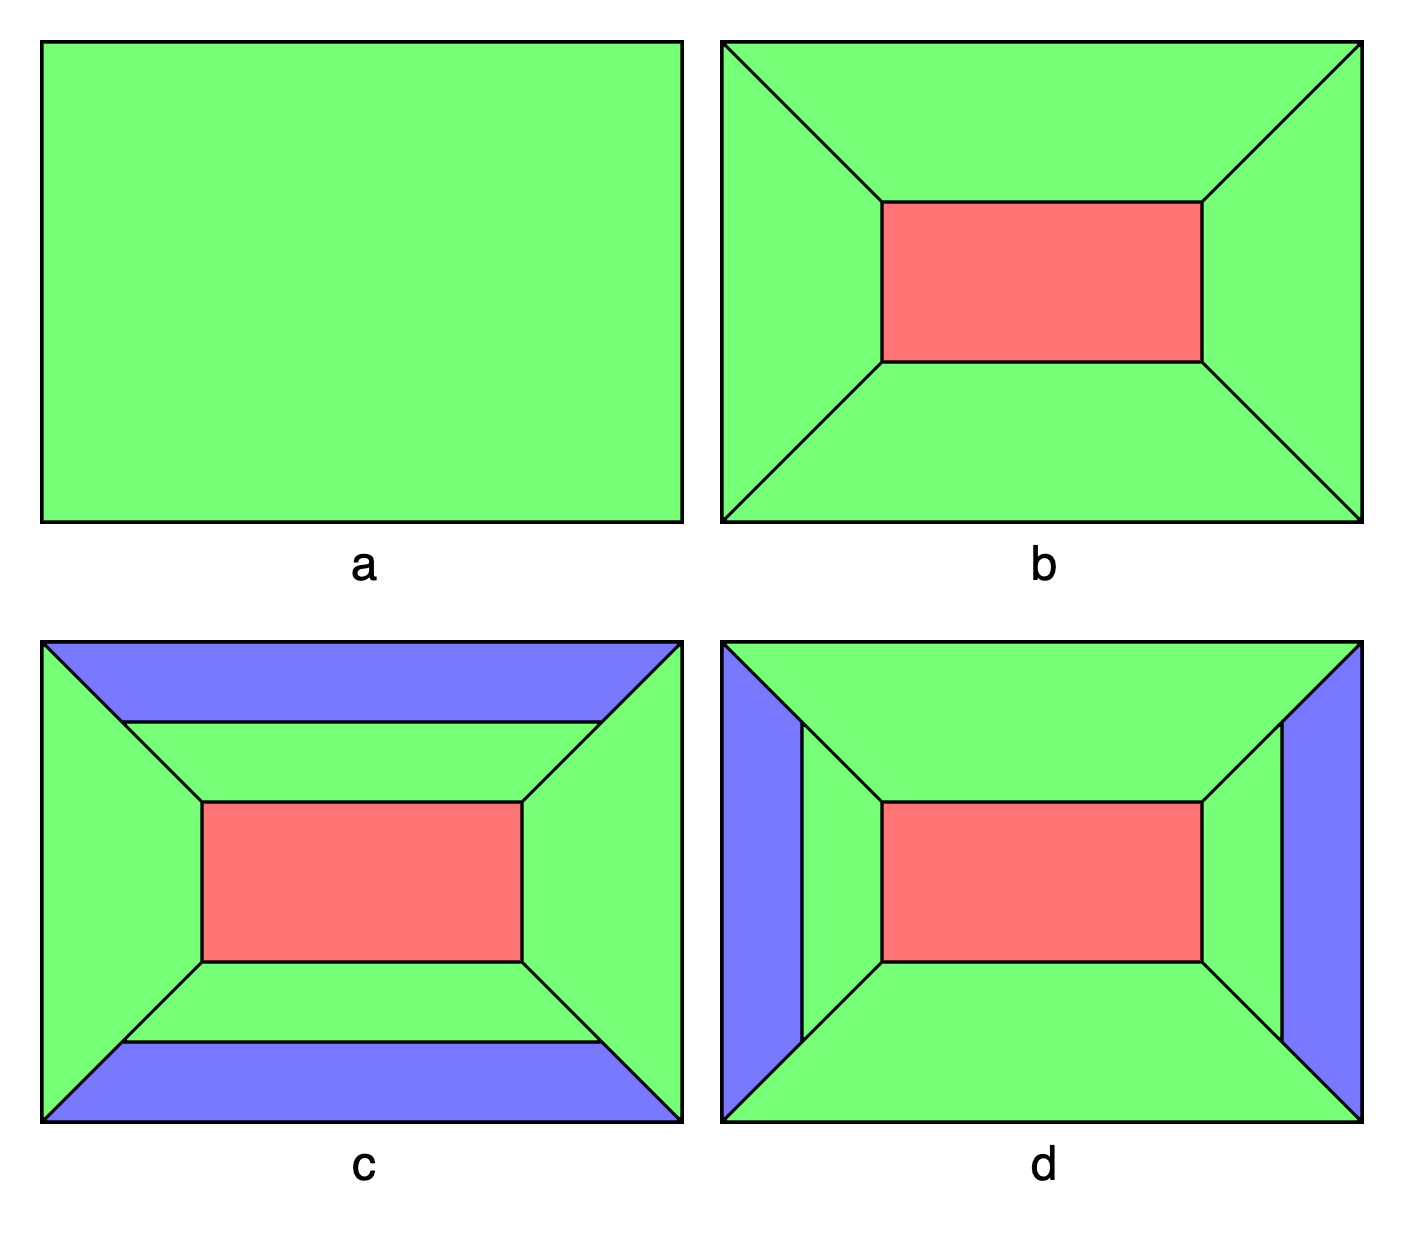
\includegraphics[scale=0.2]{img/abbildungen/Diagrammanordnunsverfahren}
    \end{center}
    \caption{Diagrammanordnunsverfahren}
\end{figure}

% Wireframes
% Agile zusammenstellen eines Dashboards
% Agiles Datenzuordnung in einem Datenflussdiagramm
% die agile Erstellung eines Datenflussdiagramms, das die Daten aus den Datenquellen verarbeitet und den Dashboards zuweist.
\subsection{Skizzen der Infrastruktur}
\label{subsec:skizzenderinfrastruktur}

% Wahl der Technologien, Tech-Stack?
% Anforderungen an die Technologien
% Umfeld etc
% Geschwindigkeit der Entwicklung
